\begin{equation*}
I = \int\limits_{-\infty}^{+\infty} [F(\lambda - \mu) - F(\lambda)]  \frac{\sin \left( \frac{\Delta_0 \mu}{2} \right)}{\pi \mu} d \mu
\end{equation*}

\begin{enumerate}

\item Если $F$~---~непрерывна при $\lambda = \lambda_0$, то $\forall \varepsilon >0 \,\overline{\Delta_0} \geq 0 \, \forall \Delta_0 \geq \overline{\Delta_0}, \, |I| \leq \xi$;

\item Пусть существует $F(\lambda_0 \pm 0)$, $F(\lambda_0 - 0) \neq F(\lambda_0 + 0)$, $F$~---~непрерывна при $\lambda \neq \lambda_0$.
\end{enumerate}

$F(\lambda) = F_c(\lambda)$~---~непрерывная часть.
\begin{equation*}
F_c(\lambda) + [F(\lambda_0 + 0) - F(\lambda_0 - 0)] \chi(\lambda - \lambda_0)\text{~---~скачок}
\end{equation*}

\subsection*{Функция $\chi$ Хэвисайда}
\begin{equation*}
\chi (t) = \begin{cases} 1, & t \geq 0; \\ 0, & t < 0. \end{cases}
\end{equation*}

\begin{figure}[h]
\begin{center}
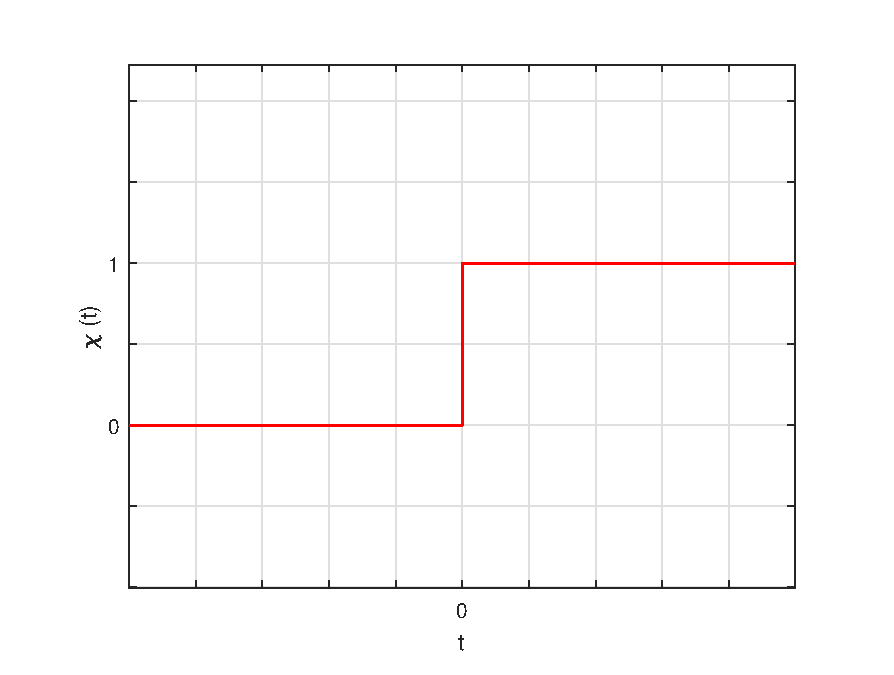
\includegraphics[width=0.6\linewidth]{ch8/ch8_fig1.eps}
\caption{Функция Хэвисайда}
\label{ch1.fig1}
\end{center}
\end{figure}

\begin{equation*}
I = \underbrace{\int \limits_{-\infty}^{+\infty}[F_c (\lambda - \mu) - F_c(\lambda)] \frac{\sin \left(\frac{\Delta_0 \mu}{2} \right)}{\pi \mu} d \mu}_{I_c} + D \underbrace{\int \limits_{-\infty}^{+\infty}[\chi (\lambda - \lambda_0 -  \mu) - \chi(\lambda - \lambda_0)] \frac{\sin \left(\frac{\Delta_0 \mu}{2} \right)}{\pi \mu} d \mu}_{I_d}
\end{equation*}

Уже было доказано, что $|I_c| \leq \varepsilon$. Теперь рассмотрим $I_d$.

\begin{equation*}
I_d = D \Bigg[ \underbrace{\int\limits_{-\infty}^{\lambda - \lambda_0} \frac{\sin \left(\frac{\Delta_0 \mu}{2} \right)}{\pi \mu} d \mu}_J - \chi (\lambda - \lambda_0) \Bigg]
\end{equation*}

Пусть $\frac{\sin \left(\frac{\Delta_0 \mu}{2} \right)}{\pi \mu} = \xi$, тогда $d \mu = \frac{2}{\Delta_0} d \xi$, $\mu = \frac{2}{\Delta_0} \xi$ то есть $\frac{d \mu}{\pi \mu} = \frac{d \xi}{\pi \xi}$.

Рассмотрим интегральный синус:
\begin{equation*}
\Si (t) = \int \limits_0^t \frac{\sin \xi}{\xi} d \xi
\end{equation*}
Он обладает следующими свойствами:
\begin{itemize}
\item $\Si$~---~нечётная функция;
\item $\Si_{t}^{'} = \frac{\sin t}{t} = 0$;
\item $t_k = \pi k$, $k \in \mathbb{N} \cup \{0\}$;
\item $\Si(+\infty) = \frac{\pi}{2}$	.
\end{itemize}

\begin{figure}[H]
\begin{center}
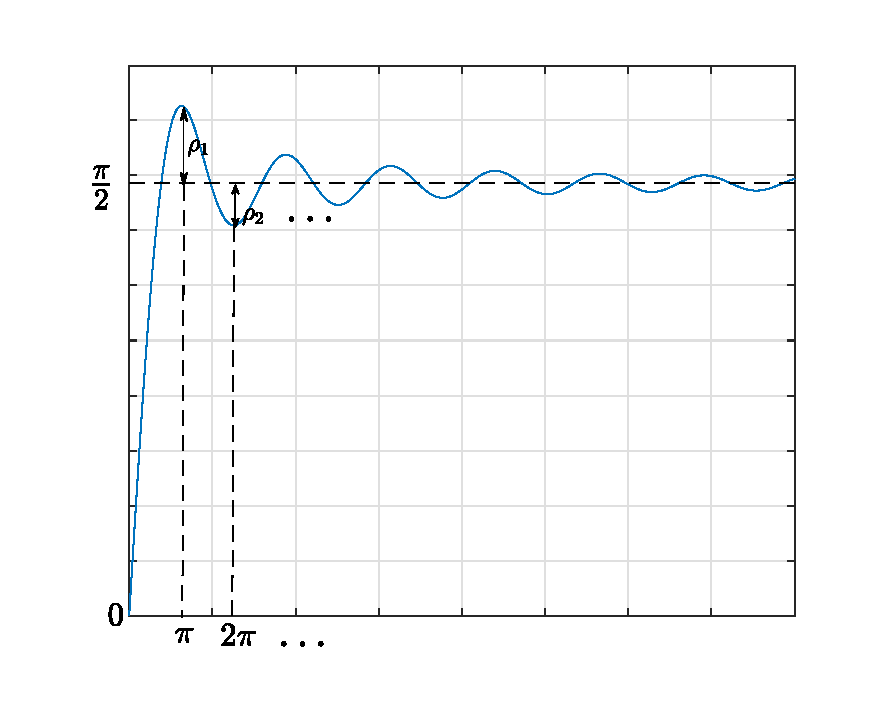
\includegraphics[width=0.6\linewidth]{ch8/ch8_fig4.eps}
\caption{Интегральный синус}
\label{ch1.fig2}
\end{center}
\end{figure}

\begin{equation*}
\Si (t) = \int \limits_0^\pi \frac{\sin \xi}{\xi} d \xi + \int \limits_\pi^{2 \pi} \frac{\sin \xi}{\xi} d \xi + \ldots + \int \limits_{\pi (k - 2)}^{\pi (k - 1)} \frac{\sin \xi}{\xi} d \xi + \int \limits_{\pi (k - 1)}^{t} \frac{\sin \xi}{\xi} d \xi
\end{equation*}

\begin{equation*}
\mu_k = \int \limits_{0}^{\pi k} \frac{\sin \xi}{\xi} d \xi
\end{equation*}
\begin{equation*}
\rho_k = \mu_k - \frac{\pi}{2}
\end{equation*}

\begin{itemize}
\item $\rho_1 \approx 0,281$;
\item $\rho_2 \approx -0,15$
\item $\rho_3 \approx 0,104$
\item $\rho_4 \approx -0,073$
\end{itemize}


$\frac{\Delta_0 (\lambda - \lambda_0)}{2} = \pi$, $\lambda - \lambda_0 = 2 \pi \Delta_0$, то есть $\lambda = \lambda_0 + \frac{2 \pi}{\Delta_0}$.


С учётом всего этого
\begin{equation*}
J = \int \limits_{-\infty}^{\frac{\Delta_{0} (\lambda - \lambda_0)}{2}} \frac{\sin \xi}{\pi \xi} d \xi = \int \limits_{-\infty}^0 \frac{\sin \xi}{\pi \xi} d \xi + \int \limits_0^{\frac{\Delta_{0} (\lambda - \lambda_0)}{2}} \frac{\sin \xi}{\pi \xi} d \xi = \frac{1}{\pi} \Si \left(\frac{\Delta_{0} (\lambda - \lambda_0)}{2}\right)
\end{equation*}

Имеем $I_d = D \left[ \frac{1}{2} + \frac{1}{\pi} \sin \left(\frac{\Delta_{0} (\lambda - \lambda_0)}{2}\right) - \chi (\lambda - \lambda_0) \right]$. \\
При $\lambda > \lambda_0$ получим $I_d \left(\lambda_0 - \frac{2 \pi}{\Delta_0} \right) = D \left[ \frac{1}{2} + \frac{1}{\pi} \left(\frac{\pi}{2} + \rho_1 \right) - 1 \right] = \frac{D \rho_1}{\pi}$.\\
При $\lambda < \lambda_0$~---~$I_d \left(\lambda_0 - \frac{2 \pi}{\Delta_0} \right) = D \left[ \frac{1}{2} + \frac{1}{\pi} \left(-\frac{\pi}{2} - \rho_1 \right) - 0 \right]= -\frac{D \rho_1}{\pi}$.

\subsection*{Эффект Гиббса}

Эффект Гиббса~---~это необычное поведение разложенной в ряд Фурье кусочно-дифференцируемой функции в точках разрыва. На иллюстрации ниже мы можем наблюдать, в чём он заключается.

\begin{figure}[H]
\begin{center}
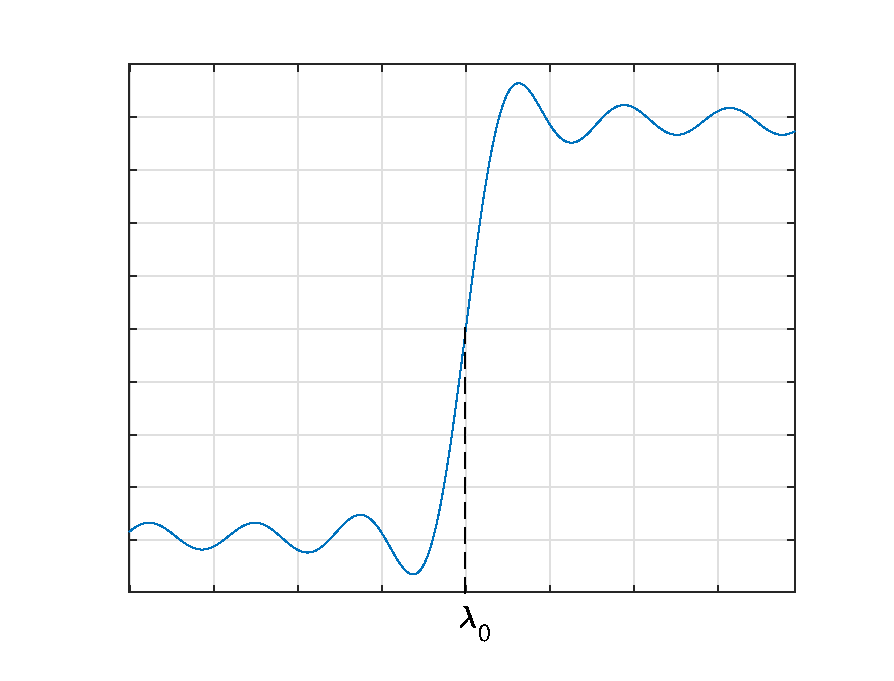
\includegraphics[width=0.6\linewidth]{ch8/ch8_fig2.eps}
\caption{Здесь можно наблюдать эффект Гиббса. То есть увеличение погрешности около точек разрыва.}
\label{ch1.fig3}
\end{center}
\end{figure}
\begin{figure}[H]
\begin{center}
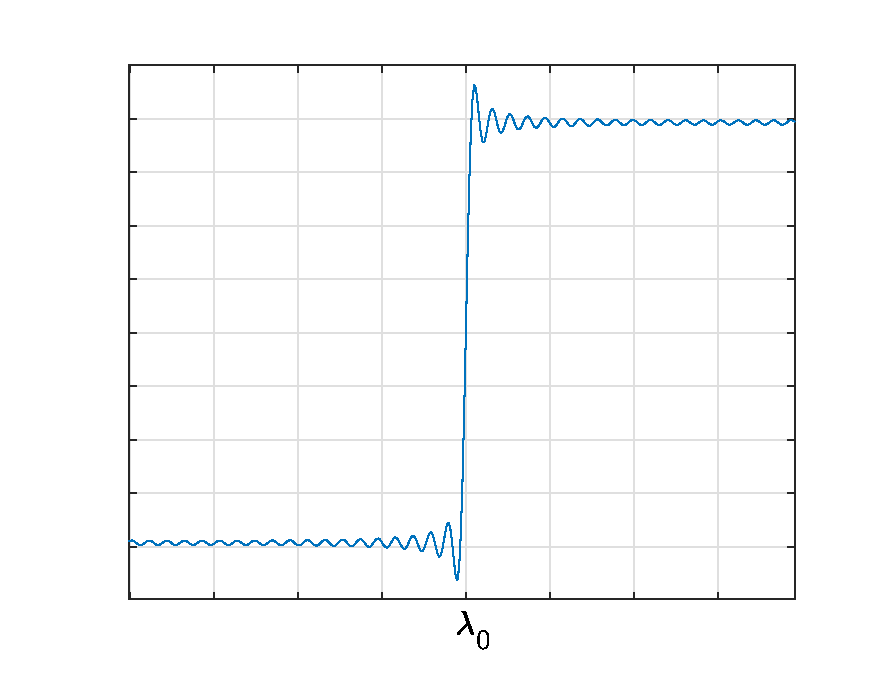
\includegraphics[width=0.6\linewidth]{ch8/ch8_fig3.eps}
\caption{При большем количестве <<волн>>}
\label{ch1.fig4}
\end{center}
\end{figure}

Данная погрешность неустранима. Это означает, что нет равномерной сходимости.

\begin{figure}[H]
\begin{center}
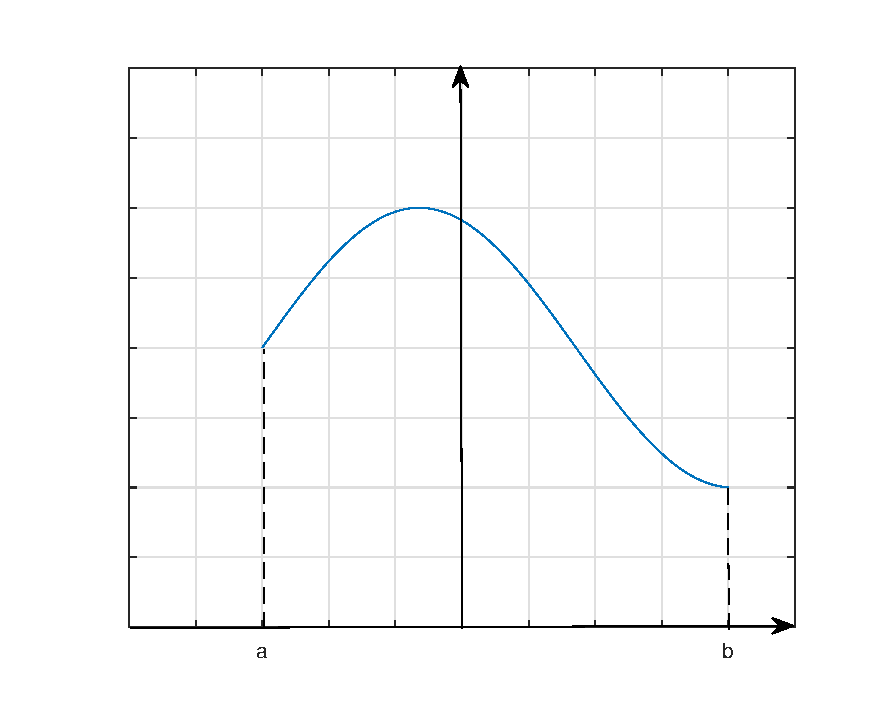
\includegraphics[width=0.6\linewidth]{ch8/ch8_fig5.eps}
\caption{Не симметричное окно}
\label{ch1.fig5}
\end{center}
\end{figure}
Имеем $N = \left\lfloor \frac{b - a}{\Delta_t} \right\rfloor + 1$, откуда следует $b \to \widetilde{b} = a + N \Delta_t$.

Что происходит с ошибкой, если окно не симметрично?

\begin{equation*}
h_{\Lambda_0} (t) = \begin{cases} 1, & |t| < \frac{\Lambda_0}{2} \\ 0, &\text{иначе} \end{cases}
\end{equation*}
\begin{equation*}
\widetilde{h}_{\Lambda_0} (t) = h_{\Lambda_0} (t - t_0)
\end{equation*}

Обычное окно, $t_0 = 0$:
\begin{equation*}
I = \int\limits_{-\infty}^{+\infty} F(\lambda - \mu) \frac{ \sin \frac{\Delta_0 \beta}{2}}{\pi \mu} d \mu - F(\lambda)
\end{equation*} 

Если же $t \neq 0$, то 
\begin{equation*}
I = \int\limits_{-\infty}^{+\infty} F(\lambda - \mu) e^{-i \mu t_0} \frac{ \sin \frac{\Delta_0 \beta}{2}}{\pi \mu} d \mu - F(\lambda) = \int\limits_{-\infty}^{+\infty} \left[ F(\lambda - \mu) e^{-i \mu t_0} - F(\lambda) e^{-i \mu t_0} \right] \frac{ \sin \frac{\Delta_0 \beta}{2}}{\pi \mu} d \mu
\end{equation*}

Рассмотрим 
\begin{equation*}
f(t) \widetilde{h}_{\Delta_t} (t) \longleftrightarrow \frac{1}{2 \pi} (F \ast \widetilde{H}_{\Delta_t}) (\lambda)
\end{equation*}
 тогда 
\begin{equation*}
\widetilde{H}_{\Delta_t}(\lambda) = \int\limits_{-\infty}^{+\infty} h_{\Delta_t} (t - t_0) e^{-i \lambda t_0} dt = e^{-i \lambda t_0} H_{\Delta_0} (\lambda)
\end{equation*}

Если $0 \in [a, b]$, то 
\begin{equation*}
\frac{1}{2 \pi}  \int\limits_{-\infty}^{+\infty} \widetilde{H}_{\Delta_t}(\mu) d \mu = h_{\Delta_0} (t - t_0) = 1, \, \text{при } t = 0
\end{equation*}

Рассмотрим следующие случаи:
\begin{enumerate}
\item $F$~---~непрерывна, тогда $\left| [F(\lambda - \mu) - F(\lambda)] e^{-i \mu t_0} \right| = |F(\lambda - \beta) - F(\lambda)|$. и следовательно $|I| \leq \varepsilon$
\item $F$ имеет разрыв. Пусть $d = D \left[  \int\limits_{-\infty}^{\lambda - \lambda_0} [\chi (\lambda - \lambda_0 - \mu) - \chi (\lambda - \lambda_0)] e^{-i \mu t} \frac{ \sin \frac{\Delta_0 \beta}{2}}{\pi \mu} d \mu \right]$.
\end{enumerate}

\section{Дискретное преобразование Фурье}

Прямое дискретное преобразование Фурье (ПДПФ):
\begin{equation*}
F_n = \sum\limits_{k = 0}^{N - 1} f_k e^{- \frac{2 \pi i n k}{N}}
\end{equation*}

Обратное дискретное преобразование Фурье (ОДПФ):
\begin{equation*}
f_k = \frac{1}{N} \sum\limits_{n = 0}^{N - 1} F_n e^{\frac{2 \pi i n k}{N}}
\end{equation*}

Удостоверимся в правильности выписанных формул.
\begin{equation*}
\frac{1}{N} \sum\limits_{k = 0}^{N - 1} \left( \sum\limits_{l = 0}^{N - 1} f_l e^{- \frac{2 \pi i n l}{N}} \right) e^{\frac{2 \pi i n k}{N}} = \frac{1}{N} \sum\limits_{k = 0}^{N - 1} f_l \sum\limits_{k = 0}^{N - 1} e^{\frac{2 \pi i n (k - l)}{N}} = \frac{1}{N}f_k N = f_k
\end{equation*}

Свойства дискретного преобразования Фурье:
\begin{enumerate}
\item Сдвиг

\begin{equation*}
f_{(k - k_0)\mod N} \longleftrightarrow F_n e^{- \frac{2 \pi i n k_0}{N}}
\end{equation*}

Сдвиг называется циклическим и по сути сводится к замене переменной (в данном случае индекса):
\begin{equation*}
\begin{aligned}
\sum\limits_{k = 0}^{N - 1} f_{(k - k_0)\mod N} e^{-\frac{2 \pi i n k}{N}} = \left\{
\begin{aligned}  k &= (k_0 + l) \mod N \\ k &= k_0 + l + q_ l N \end{aligned} \right\} = \sum\limits_{k = 0}^{N - 1} f_l &e^{-\frac{2 \pi i n (k_0 + l + q_lN}{N}} = \\ &=\sum\limits_{k = 0}^{N - 1} f_l e^{-\frac{2 \pi i n l}{N}}  e^{-2 \pi i n q_l}  e^{-\frac{2 \pi i n k_0}{N}}
\end{aligned}
\end{equation*}

\item Свёртка

В данном случае она тоже будет называться циклической или круговой. Пусть имеем
\begin{equation*}
\begin{aligned}
&f_n \longleftrightarrow F_n\\
&g_n \longleftrightarrow G_n
\end{aligned}
\end{equation*}
тогда 
\begin{equation*}
h_k = (f \ast g)_k = \sum\limits_{l = 0}^{N - 1} f_l g_{(n - l) \mod N} \longleftrightarrow F_n \cdot G_n
\end{equation*}
\end{enumerate}